%%automated verification
\textcolor{red}{What is the relation between CPS and PV? We should make it clear already in the beginning...}
Cyber-Physical Systems (CPS) are engineered systems, which are built from, and depend upon, the seamless integration of computational and physical components~\cite{NSF2015,ChavesIBCF19,iet-cps.2018.5006}. During operation, such components must frequently adapt to the operating environment changes (dynamics of the physical processes) faced at run-time. They must be able to continue to behave in a controlled and safe way, thus posing novel technical challenges for the software engineering of services and applications for CPS~\cite{Metzger2014}. Software pervasiveness in CPS places new challenges; in particular, highly dynamic environments, rapidly changing requirements, unpredictable and uncertain operating conditions demand new paradigms for software design~\cite{Filieri2015}.

While some research efforts do exist to enhance and optimize the software development processes for CPS, further investigation and discussion of better and more effective models are still needed in practice~\cite{Al-Jaroodi2016}. Among the opportunities for enhancements in the software development processes for CPS, there exists the need for developing new techniques and tools to support CPS requirements gathering and analysis to synthesize \textit{correct-by-construction} implementations of CPS. These techniques need to deal with predefined requirements enforced by nature and inherited constraints of the target CPS. Besides, they should be able to provide verification and validation mechanisms for completeness, correctness, and consistency~\cite{Al-Jaroodi2016}. Uncertainty and variability, at the same time, can be dealt with formal verification~\cite{NESSI}. Energy production, distribution, and optimization are all CPS problems~\cite{UC}. 

Lack of access to clean and affordable energy is considered a core dimension of poverty~\cite{Hussein2012}. Nevertheless, the world is progressing; in particular, the number of people without electricity access fell below 1 billion threshold for the first time in 2017~\cite{IEAweo2018}. The share of people without access to electricity from Africa is 58\%, while 19\% of the share comes from developing Asia, and 31\% from Latin America~\cite{IEAweo2018}. Numbers from Brazil show the aim to electrify 270 isolated places and 2.7 million people until 2023~\cite{EPE2018}. 
Furthermore, there exists a close relationship between the lack of energy and the low HDI (Human Development Index) of those localities~\cite{Coelho}. Therefore, increased access to energy allows economic growth and poverty alleviation \cite{Karekesi}.

The use of the power generation technology with renewable energy source is developing rapidly due to the industrial development~\cite{Yatimi}. The renewable energy leads to an advance all over the world by protecting the environment: it is clean (low greenhouse gas emissions), operating silently, long lifetime, low maintenance, absence of fuel cost and inexhaustible~\cite{Noroozian}. Renewable energy, and particularly the power generation from solar energy using photovoltaic (PV) panels, has emerged as an alternative to fossil or nuclear fuel generation. 

Among the options of renewable sources, there exist hydro, wind, and solar PV. According to~\cite{SEIA} and~\cite{Chauhan}, solar is the most abundant source of renewable energy on earth. In solar PV systems, solar radiations are captured from the sun and turned into electricity using solar PV cells made of silicon and other materials.

Only a niche market a few years ago, solar PV systems are now becoming a mainstream electricity provider, with an increase of approximately 50\% from 2016 to 2017 in terms of new installations of PV~\cite{EPIA}. However, this growth is not driven by stand-alone systems.

However, in order to provide universal electricity, decentralized systems led by solar photovoltaic (PV) in off-grid and mini-grid systems will be the lowest-cost solution for three-quarters of the additional connections needed. Grid extension will be the standard, especially in urban areas~\cite{IEAweo2018}.

The PV cell in a solar PV system, as defined in \cite{Rawat}, is a semiconductor device, which directly converts solar radiation into electrical energy. Apart from PV modules, the PV systems consist of a battery bank, controller, and inverter, plus the load.
%The definition of energy access usually includes both electricity access and access to modern fuels for cooking and heating, in order to replace traditional biomass. 
%
%However, to the best of our knowledge, this work can be the first work to perform automated verification of a stand-alone solar PV project solution.  
%
%The increase in a number of PV systems installed all over the world brings the need for proper modeling and simulation tools for researcher and practitioners involved in their application.

The increase in the number of PV systems installed all over the world brings the need for proper modeling of those equipment and simulation tools for researchers and practitioners involved in their application. 

Moreover, the optimum sizing of these devices is essential for reliable operation. Therefore, these systems need to be appropriately designed according to the site, the land area available, load requirement, load pattern, environmental conditions, and economics in order to utilize available resources efficiently and economically~\cite{Rawat}.

%-------------------------------------------------
\section{Problem's Definition}
%-------------------------------------------------

In order to address different aspects of a solar PV project, there exists a myriad of public domain and commercial software available, such as RETScreen, HOMER, PVWatts, SAM, and Hybrid2 \cite{Pradhan,Swarnkar,NRELDobos,NRELBlair,Mills}; and even general-purpose simulation tools such as PSpice, and MATLAB/Simulink package \cite{Gow1999,Benatiallah2017}. According to~\cite{Brooks}, the capabilities of these tools range from simple solar resource and energy production estimation to site survey and system design tools, to sophisticated financial analysis software (with optimization). Some tools also provide support to rebate program applications and tax incentives (specific to each country or region), while other programs and worksheets focus on the technical aspects of system sizing and design.  
%
Manufactures and integrators have yet their proprietary software to perform various system sizing~\cite{Zhou2010}, with the drawback of including just their products among the possibilities of choice, which restricts their solution. 
%
%PV systems can be classified into grid-connected and stand-alone systems. At this proposal, only off-grid or stand-alone systems will be considered. The utilization of solar energy in off-grid mode has the potential to meet the energy need for remote rural areas of developing countries.  
However, public domain and commercial software or even proprietary tools are based on running experiments in simulation models. Simulation has the advantage of being cheap (if compared to testing in real systems) and can be employed before the system design is concluded. However, it has the drawback of an incomplete coverage since the verification of all possible combinations, and potential failures of a system is unfeasible~\cite{ClarkeHV18}.

Formal methods based on model checking offer a great potential to obtain a more effective and faster verification in the design process~\cite{ClarkeHV18}, including, for example, applications to CPS~\cite{Abateetal2017,AbateBCCDKK17,Bessa,ChavesBCKF17}, with behavior that is, in principle, well determined. 
Any system type can be specified as computer programs using mathematical logic, which constitutes the intended (correct) behavior; then, one can try to give a formal proof or otherwise establish that the program meets its specification~\cite{DBLP:journals/sttt/GadelhaIC17}. User or project requirements can be added during the creation of the formal model to be verified~\cite{Trindade,TrindadeDJISC17}. 
%
This research area is referred to as formal methods~\cite{Clarkeetal}, which aim to establish system correctness with mathematical rigor. 
In recent decades, research in formal methods has led to the development of up-and-coming verification techniques that facilitate the early detection of flaws in order to ensure the correctness of the system, including programming languages such as C/C++ and Java~\cite{esbmc2018,RamalhoFSMC013,CordeiroKKST18}. 

Model-based verification techniques are based on models that describe the possible system behavior in a mathematically precise, and unambiguous manner. Thus, such problems as incompleteness, ambiguities, and inconsistencies, which generally are discovered only in later stages of the design, can be detected in advance, as described by \cite{Trindade,TrindadeDJISC17}. 
Model checking algorithms can then verify the system model by systematically exploring all its states to check whether the given system meets the requirements.
%
%Formal methods, alternatively, provide facilities for the modeling of each component of any complex system~\cite{Hall1990}. 
%

%automated synthesis
However, optimization of PV systems is not a recent topic; since the $90$'s different techniques using a wide variety of criteria to find ultimate combinations for design parameters, based on intuitive, numerical, and analytical methods were developed and evaluated~\cite{Applasamy2011}. An ideal combination of any PV system is made by the best compromise between two considered objectives, which is \textit{power reliability} and \textit{system cost}~\cite{Alsadi2018}.
 
However, formal methods based on \textit{symbolic model checking} and its application to synthesize PV systems have not been further explored in literature, which could offer a great potential to obtain a more effective design process to PV systems~\cite{ClarkeHV18}.

%----------------------------------------------
\section{Objectives}
%----------------------------------------------

The main objective of this thesis is thus to propose and evaluate the use of formal methods in solar PV systems, using a computer science method to solve specific issues of the electrical engineering area. \textcolor{red}{This sentence is too long and unclear...} In particular, we focus on automated verification by model checking, on stand-alone solar PV systems that is most adequate to rural areas of developing countries, on the need to validate and optimize those systems, on evaluating different state-of-art symbolic software verifiers (and solvers) with the goal of obtaining the best performance in our verification back-end, on applications written in ANSI-C that are platform-independent; and we do not perform code modification on the verifiers or solvers, we use it as available by their developers. We further evaluate our proposed solution by comparative with commercial simulation tool and by data collected from real PV systems deployed at riverside communities.
%More specifically we will:
%The thesis produces a methodological research with innovative value regarding the first use of automated synthesis for optimal sizing of solar PV systems.

\textcolor{red}{A PhD thesis is not simply the application of methods and development of tools. Please rephrase this sentence.}
This Ph.D. thesis has the novelty of applying automated verification method to solar PV systems. The result is the development of two software: one to perform automated verification and validate the solar PV systems behavior, and another one to produce the optimal sizing of solar PV systems through automated synthesis program.

In this study, a mathematical model of each component of a stand-alone PV system, as panel solar, charge controller, batteries, inverter, and electrical load is used for formal verification. The behavior of each system component can be analyzed and observed with the support of those formal models, as a joint operation of the components, which in this case represents the operation of the solar PV system itself. The project requirements, as battery autonomy and power demand, besides weather conditions, as solar irradiance and ambient temperature, are provided to the proposed tool and automatically verified during the formal process. The model checking tool reports in which conditions a system does not meet the user requirements. A key benefit to this approach is that it helps in the detection of flaws in the design phase of system development, thereby considerably improving system reliability~\cite{Akram2018}. 
%Those programs are viewed as mathematical objects, and the use of 
%Bringing this technique to solar PV systems, i
%Instead of finding a bug or a software inconsistence, t
%Here it will be verified a stand-alone PV system, with all their components modeled mathematically,   
%Among the non-deterministic variables considerated, is it worth to mention environmental issues (like solar irradiance, and temperature), and the variation of the electrical load (power consumption) or the battery' state of charge, as shown in Fig.\ref{fig:flowchartgeneral}.
\textcolor{red}{This paragraph is too long and unclear...}
The implementation of the proposed tool is carried out by means of an algorithm implemented using the C programming language, which is executed by three state-of-the-art model checkers to formally verifying PV designs, in order to evaluate performance and correctness: the C Bounded Model Checker (CBMC)~\cite{Kroening}, the Efficient SMT-based Bounded Model Checker (ESBMC)~\cite{esbmc2018}, and the Configurable Program Analysis Checker (CPAchecker).
%three the efficient SMT-based bounded model checker (ESBMC)~\cite{esbmc2018}. %, which allows one to incrementally verify a PV system as an imperative program using a fragment of decidable first-order theories~\cite{DBLP:books/daglib/0019162}.

Related to \textbf{automated synthesis} method and the optimal sizing of stand-alone PV systems, this thesis presents the development of a variant of counterexample guided inductive synthesis (CEGIS) that uses commercial equipment data, user requirements and weather conditions as input. Given a correctness specification $\sigma$, the proposed method uses that as a starting point and then iteratively produces a sequence of candidate solutions that satisfy $\sigma$, related to power reliability. In particular, in each iteration, we synthesize the sizing of stand-alone PV systems, but that may not achieve the lowest cost. The candidate solution is then verified via symbolic model checking with a lower bound that serves as the minimum cost of reference; if the verification step does not fail, the lower bound is adjusted. If it fails, then a counterexample is provided with an optimal sizing that meets power reliability and system cost. Note that in this study, the focus is not on new criteria or even optimization objectives. Instead, the novelty relies on a practical approach on the pursuit of the optimal solution of PV systems using formal methods, which outperforms existing state-of-the-art simulation tool.


%----------------------------------------------
\section{Outline of the Solution}
%----------------------------------------------
%\textcolor{red}{you should briefly describe here the outline of your solution. As example, take a look at \url{https://ssvlab.github.io/lucasccordeiro/papers/phd\_thesis\_cordeiro.pdf.}}

Our approach deals with the theoretical and pragmatic aspects of using model checking in stand-alone solar PV systems in order to tackle two issues: validation of a designed system and optimal sizing. Validation when a sized system must be evaluated in order to define if it meets the design requirements and user needs; and optimization when there are just the requirements and the PV system is not sized, or then the user tries to obtain a better solution that he or she has. We thus develop algorithms and the corresponding tools; moreover, we evaluate them using a comparative process \textcolor{red}{what do you mean by a ``comparative process''?} in several case studies with specialized simulation tools and real data from deployed PV systems.

Fig.\ref{fig:validation_outline} outlines the proposed solution to perform the validation of stand-alone solar PV systems via automated verification. Fig.\ref{fig:optimization_outline} illustrates the proposed solution to obtain the optimal sizing of stand-alone solar PV systems via automated synthesis. We pictured here only a summary of each phase of our proposed approach, with highlights to the input parameters, the outputs for the validation, or the optimal size of the solar PV system; more details are presented in the next chapters. Moreover, the illustrations show the methodological approach related to comparative result analysis, employing our approaches, commercial software tool, and data from real PV systems deployed in the field.

\begin{figure}[h]
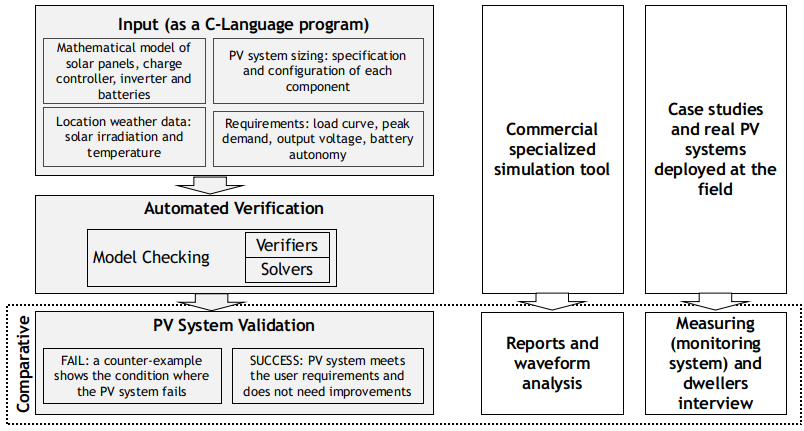
\includegraphics[width=0.85\textwidth]{verification_outline2.png}
\centering
\caption{Proposed validation of PV systems via automated verification.}
\label{fig:validation_outline} 
\end{figure}


\begin{figure}[h]
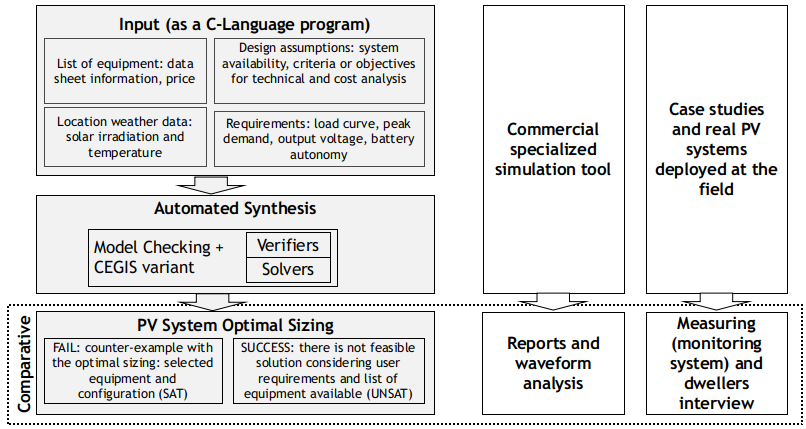
\includegraphics[width=0.85\textwidth]{optimization_outline2.png}
\centering
\caption{Proposed optimal sizing of PV systems via automated synthesis.}
\label{fig:optimization_outline} 
\end{figure}

Note that it is out of our scope to perform code modification on the verifiers or the solvers used during the automated verification or automated synthesis steps of our approach. \textcolor{red}{why is it out of scope? You need to explain here.}

%----------------------------------------------
\section{Contributions}
%----------------------------------------------

% Firstly, we describe a modular modeling of each component of a PV system by means of mathematical models that can be encoded into fragments of first-order theories supported by software model checkers. Secondly

\textcolor{red}{The beginning of this sentence is weird...}
Associated with \textbf{automated verification}, this thesis makes three main contributions. 
\textbf{First}, we propose an algorithm written in the C programming language, which implements the automated verification method to formally check the sizing and the operation of a given stand-alone PV system. 
\textbf{Second}, we evaluate the verification method by comparing three state-of-the-art model checkers in five real case studies. 
\textbf{Third}, experimental results show that this proposed approach can find subtle design errors in stand-alone PV systems, which are not easily detected by other approaches based on simulation. 
%
%The framework provided at this paper outlines the requirements, the process and the mathematical modeling to perform automated formal verification of a stand-alone PV system, using the satisfiability modulo theories (SMT)-based verification method.

\textcolor{red}{The second and third contributions are long and tough to read. I don't understand them.}
And linked to \textbf{automated synthesis}, our work makes more three original contributions: \textbf{First}, it is the first application of a sound and automated formal synthesis approach, which can provide accurate results of optimal sizing of stand-alone PV systems; 
\textbf{Secondly}, we propose a variant CEGIS method with striking differences of how the {\sc Synthesize} and {\sc Verify} phases work together, with the abolition of the feasible solution candidate vector and the use of an incremental, iterative loop to reach the optimal cost solution of the system; and 
\textbf{Thirdly}, experimental results with seven case studies show that formal synthesis approach qualitatively outperforms an existing state-of-the-art simulation tool. Our solution is far detailed and closer to the commercial reality (real PV systems) than the solution presented by simulation.

%three major contributions. 
%\textbf{First}, the use of automated symbolic verification methods in electrical systems was uncommon in recent prior studies~\cite{abs-1811-09438}, and specifically their use in synthesizing optimal PV sizing is unprecedented. Here, a list of PV components (i.e., PV panels, charge controllers, inverters, and batteries) can be fed to the proposed synthesis method together with the user requirements and environment constraints, and the proposed synthesis algorithm based on symbolic model checking can find the optimal solution in technical and economical terms. 
%\textbf{Second}, we evaluate different state-of-art symbolic software verifiers with the goal of obtaining the best performance in the verification back-end for synthesizing optimal PV systems, thereby being the first work that performs this type of evaluation. 
%\textbf{Third}, the experimental results show that the proposed synthesis method is an effective and efficient approach on the pursuit of the optimal solution of PV systems using formal methods, which outperforms existing state-of-the-art simulation tool. As a result, this thesis marks the first application of a sound and automated formal synthesis approach able to provide accurate results of optimal sizing of stand-alone PV systems. Thus, this research considerably advances the state-of-the-art in applied energy over the last two decades with the goal of optimally designing PV systems.
 
%---------------------------------------------- 
\section{Related Work}
%----------------------------------------------

Here we discuss only the use of formal methods on electrical systems in general since currently there exists no use of it or even program synthesis to obtain the optimization of PV sizing.

The conversion of the traditional power grid into a smart grid, a fundamental example of a CPS, raises many issues that require novel methods and applications. In $2012$, a Chinese smart grid implementation was considered as case study to address the verification problem for performance and energy consumption~\cite{Yukseletall2012}. The authors employed a stochastic model checking approach and presented a modeling and analysis study using PRISM, which is a probabilistic model checker~\cite{KwiatkowskaNP11}. \textcolor{red}{This sentence is too long...} The focus of this study was on how CPSs integrate information and communication technology functions to the physical elements of a system for monitoring and controlling purposes; here, the authors employed automated verification of certain quantitative properties of the system, as probability of node failure in the long run, impact of repair service on the failure risk, and expected energy consumption, without any interest in power generation or even solar PV systems.

In $2015$, an automated approach for applying Monte-Carlo simulation to power system protection schemes presented limitations of incomplete coverage of all possible operating conditions~\cite{Sengupta2015}. The authors proposed an automated simulation-based verification technique to verify the correctness of protection settings efficiently using a hybrid automata-temporal-logic framework. The initial focus was on relay operations and test-case generation to ensure the early detection of design errors. However, this study was limited to power system protection and did not deal with electricity generation or even solar PV systems.

Other related studies from $2015$ include a framework named Modana to achieve an integrated process from modeling with SysML/MARTE to analysis using statistical model checking for CPS in terms of non-functional properties such as time and energy~\cite{Cheng2015}. In order to demonstrate Modana's capability, the authors modeled energy-aware buildings as a case study and discussed the analysis of energy consumption in different scenarios. The focus here is on smart buildings and HVAC (heating, ventilation, and air conditioning) systems. This research, however, did not address the design and verification of solar PV systems. 
 
In $2017$, a researcher suggested the application of formal methods to verify and control the behavior of computational devices, interacting over a shared and smart infrastructure~\cite{Abate2017}. The author discussed the aggregation of large populations of thermostatically-controlled loads and PV panels, and the similar problems of energy management in smart buildings, of demand-response on smart grids, and respectively of frequency stabilization and grid robustness. The focus was on controlling the behavior of components, thereby verifying the given smart grid as a ``system of systems'' within the context of "internet of things". The author, however, used an approximate model checking of stochastic and hybrid models.

In $2018$, a verification methodology was proposed for the Cyber-Physical Energy Systems (CPES) with applications to PV panels and its distributed powerpoint tracking~\cite{Driouich2018}. This approach relied on representing the unpredictable behavior of the environment to cover all possible feasible scenarios. The simulation results obtained by JModelica covered the system's complete dynamic behavior; however, it was evident the time-consuming issue with almost three days of computer effort to verify the design space of one operation hour of the PV panels behavior. This related study did not include other components of a stand-alone solar PV system.

Another work from $2018$ was the approach to model smart grid components using a formal specification. The authors used a state-based formal specification language named Z; they demonstrated the application of Z to four smart grid components~\cite{Akram2018}. The presented formal specification can be considered as a first step towards modeling of smart grids using formal methods. The starting point of this study was that a smart home can be considered as an integrated system consisting of various objects and systems, which communicates and interacts with each other. This approach is based on Petri nets and is under the assumption that modeling the smart home leads to a clear understanding of the overall behavior of the smart grid.

However, prior studies did not deal with formal verification of a complete stand-alone PV system (with batteries, charge controller, and power inverter) or even solar PV systems optimization. Formal methods based on \textit{symbolic model checking} and its application to synthesize PV systems are still unexplored in literature. Moreover, it is precisely in those gaps that this thesis focuses on.

%----------------------------------------------
\section{Thesis Organization}
%----------------------------------------------

This introduction has outlined the context, motivation, and problem addressed by this thesis and the objectives, solution, and contributions of the research. The remainder of the chapters of this thesis are organized as follows:

Chapter '~\nameref{chap:background}' gives the theoretical basis on formal methods, formal verification, automated verification, solar PV systems, design and validation of PV systems, program synthesis, and the mathematical modeling. 

Chapter '~\nameref{chap:automatedverification}' presents the automated formal verification technique, the experimentation details, and the results obtained with the tool created using this new method of PV systems validation. 

Chapter '~\nameref{chap:automatedsynthesis}' presents the automated synthesis technique from computer science and its application to obtain the optimal sizing of stand-alone solar PV systems, with details of the experimentation, and the results using the tools created to compare this new technique with simulation tool and from data collected from fieldwork. 

Chapter '~\nameref{chap:conclusions}' presents the main contributions, future work directions and concluding remarks.

\textcolor{red}{This sentence is unclear...}
~\autoref{chap:publications} presents a list of papers that were written during the thesis elaboration and the status of every submission until the date of this document.

~\autoref{chap:tools} depicts the tools created during the PhD process to implement and validate the two scientific methods of the thesis (and how to use it).